\documentclass{article}
\usepackage[utf8]{inputenc}
\usepackage{geometry}
\usepackage{graphicx}
\usepackage{pgfplots}
\usepackage{amsmath}
\usepackage{amssymb}
\usepackage{amsfonts}
\usepackage{mdframed}
\usepackage{amsthm}
\usepackage{physics}
\usepackage{derivative}
\usepackage{hyperref}
\renewcommand{\theenumi}{\roman{enumi}}

\geometry{a4paper, left=2cm, right=2cm, top=1cm, bottom=2cm}

\pgfplotsset{compat=1.18}
\begin{document}

\begin{minipage}{0.7\textwidth}
    \small \textbf{INTRODUCCIÓN A LA FÍSICA CUÁNTICA}  \\
    \small {Facultad de Ciencias, Universidad Nacional Autónoma de México} \\
    \small {Profesor: Zaahel Mata Pinzon} \\
    \small {Ayudante 1: José Andrés Carlos López}\\
    \small {Ayudante 2: Luis Enrique Soria Rubio}\\
    \small {Fecha de entrega: 21 de Febrero de 2024} \\
    \small {Nombre completo: Andrés López González} \\
    \small {Tarea número I}
\end{minipage}
\hfill
\begin{minipage}{0.12\textwidth}
    
\includegraphics[width=\linewidth]{logo_universidad}
\end{minipage}

\section*{Problemas}

\begin{enumerate}
    \item (2 pts) Supón que lanzamos 2 dados.
    \begin{enumerate}
        \item[a)] ¿Cuál es la probabilidad de que la suma sea par?
        \textit{Es facil comprobar que existen 18 formas de llegar a un número par a partir de la suma de dos dados, para ello nótese que para un dado de cara con valor fijado en un número par al sumarse con otro par dará un número par, e.j: denotamos la pareja ordenada de dados $(d_1,d_2)$ tal que $d_1=d_{fix}=2n :n\in \{ 1,2,3 \}$, vease que si $d_1$ es sumado por un par (2, 4, 6) el resultado será otro par, análogamente con los impares sabemos que la suma de 2 impares es un par ($(2n-1) + (2m-1) = 2(n+m-1)$, de donde ($n+m-1\in\mathbb{N}$)). Dado que tenemos 3 casos pares para cual sea valor fijo de un dado, entonces el número de formas de llegar a un número par con la suma de dos dados es representado algebráicamente como $6 \times 3=18$. Y esto era inmediato de ver "a mano" viendo la segunda table que se nos proporcionó en la fase teórica. Ahora como tenemos 6 "primeros estados" que se ramifican en 6 cada uno, el total de resultados es 36 (sin discriminar en este contexto que se repitan). i.e. la probabilidad de un número par es
        $$\sum_{d_i \in D:d_i=2n (n\in\mathbb{N})} \frac{E_{d_i}}{S} = \frac{18}{36} = \frac{1}{2}$$. Dejaré un poco de lado el formalismo de cosas triviales porque es dificil de codificar en latex xd}
        \item[b)] ¿Cuál es la probabilidad de que la suma sea menor a 5?
        \textit{Buscamos la probabilidad $P(d_i<5)$, esto se ve como $P(d_i):d_i\in\{ ...,0,1,2,3,4\}$. Descartando los casos imposibles acorde al espacio muestral y las condiciones iniciales tenemos que la probabilidad se expresa como $P(2)+P(3)+P(4)=6$ (esto se obtiene solo viendo cuantas veces aparecen estos 3 números en la tabla). Como ya conocemos el número total de resultados $S$, obtenemos que $P(d_i<5) = \frac{6}{36} = \frac{1}{6}$}
        \item[c)] ¿Cuál es la probabilidad de que la suma sea exactamente 5?
        \textit{Contamos las veces que aparece el 5 en la tabla, nótese que solo existen 4 formas de que la suma de dos dados de exactamente 5. Entonces $P(d_i=5) = \frac{4}{36} = \frac{1}{9}$}
    \end{enumerate}
    
    \item (2 pts) ¿Cuál es la probabilidad de que se observen menos de 3 caras en 12 lanzamientos de la moneda?
    

    \item (3 pts) Supongamos que el 13\% de las personas son zurdas. Si seleccionamos a 5 personas al azar, encuentra la probabilidad de cada uno de los siguientes resultados:
    \begin{enumerate}
        \item[a)] El primer zurdo en la quinta persona elegida.
        Ilustraremos la probabilidad con un diagrama de arbol de ramificaciones no homogeneas simplificado.
        \begin{figure}[h]
            \centering
            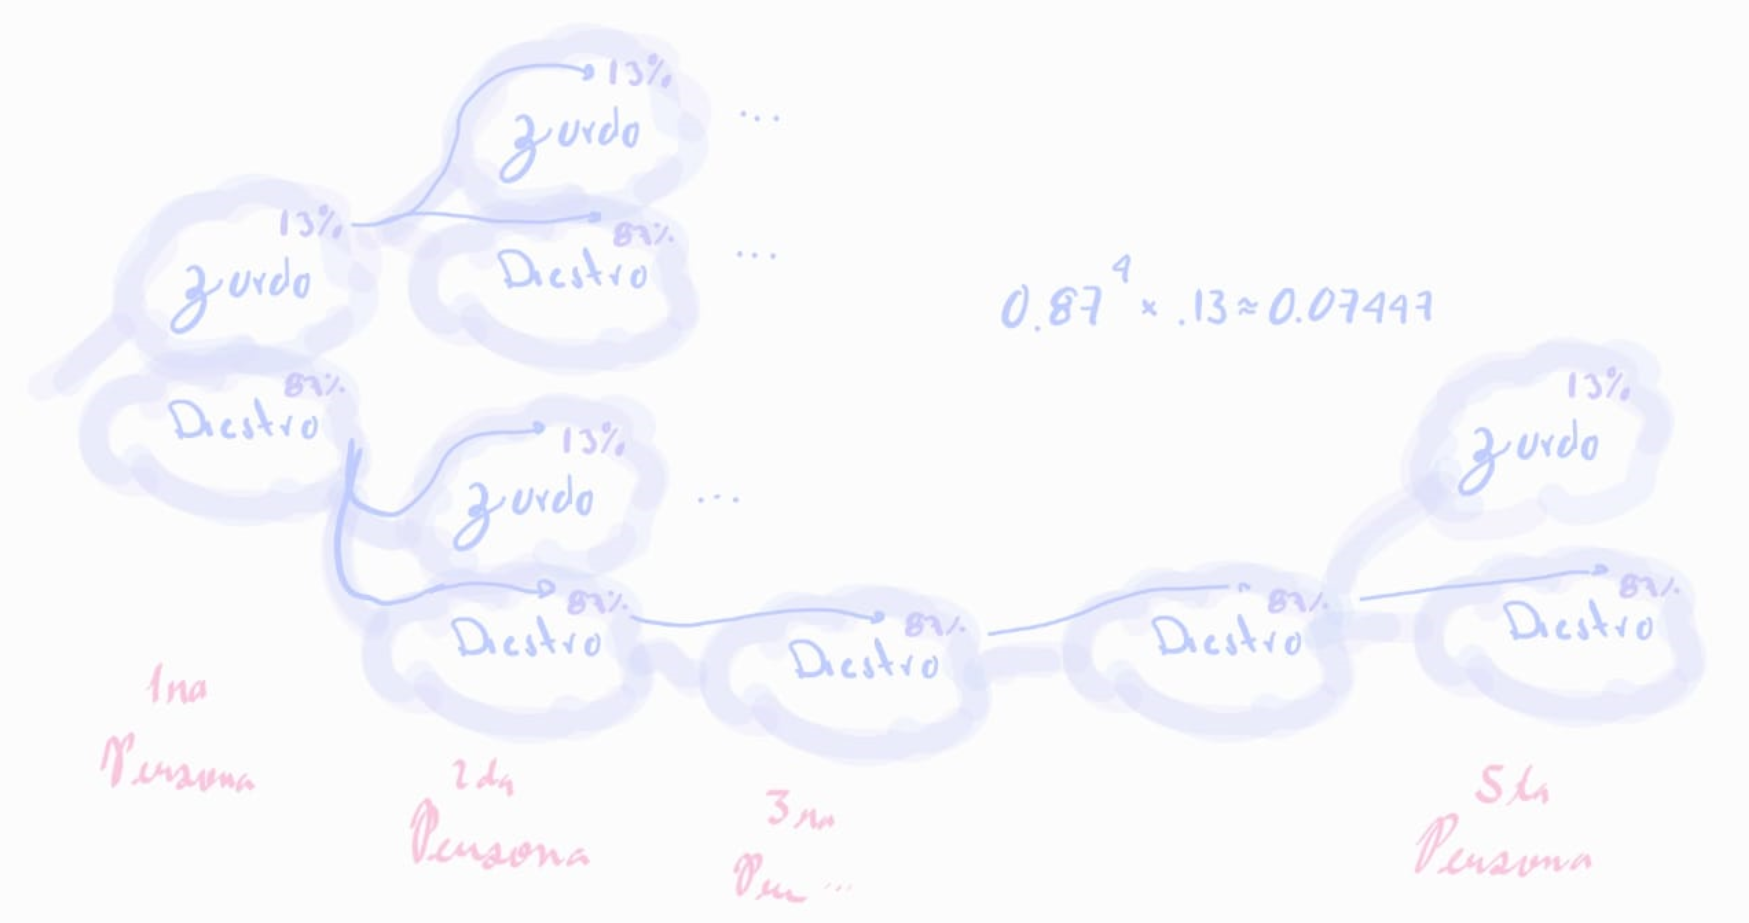
\includegraphics[width=0.75\linewidth]{pZqta.png}
            \caption{Diagrama de arbol no homogéneo del planteamiento 3a}
            \label{fig:enter-label}
        \end{figure}
        Nótese que cada que elegimos que la siguiente persona sea no zurda, la probabilidad decae, pues a pesar de ser la opción más probable, existe el caso del 13\% que sea zurdo. Vemos el caso de que la persona elegida no sea zurda
        \item[b)] Existen exactamente 2 zurdos en el grupo.
        \item[c)] Existe al menos un zurdo en el grupo.
        \item[d)] No existen más de 3 zurdos en el grupo.
    \end{enumerate}

    \item (2 pts) Para encontrar la probabilidad de obtener exactamente dos 3's en 5 lanzamientos de un solo dado, ¿qué hay de incorrecto con la estrategia de utilizar la regla de multiplicación para encontrar la probabilidad de obtener dos 3's, seguidos de tres no-3's, la cual es:
    \[
    \frac{1}{6} \cdot \frac{1}{6} \cdot \frac{5}{6} \cdot \frac{5}{6} \cdot \frac{5}{6} = \left(\frac{1}{6}\right)^2 \cdot \left(\frac{5}{6}\right)^3
    \]

    \item (3 puntos) La Tabla de Galton (Figura 1) es un dispositivo que ilustra el concepto de distribución binomial y la aproximación a la distribución normal. Consiste en un tablero vertical con filas de clavos dispuestos en forma triangular. Al soltar una canica desde la parte superior, esta choca con los clavos y se desplaza aleatoriamente hacia la derecha o hacia la izquierda hasta llegar a uno de los compartimentos en la base.
    \begin{enumerate}
        \item[a)] Si una cuenta rebota hacia la derecha \( k \) veces en su camino hacia abajo (y hacia la izquierda en las filas restantes), termina en el contenedor \( k \)-ésimo contado desde la izquierda. Numerando las filas de clavos en un tablero de Galton como \( n \), ¿cuál será el número de caminos al contenedor \( k \)-ésimo en la parte inferior?
        
        \item[b)] Supongamos que nuestra Tabla de Galton tiene 10 filas de clavos y 13 contenedores en la base. Cada vez que una canica choca con un clavo, tiene la misma probabilidad de desplazarse hacia la derecha o hacia la izquierda. ¿Cuál es la probabilidad de que una canica termine en el contenedor central?

        \item[c)] Si soltamos 100 canicas, ¿cuántas esperaremos que terminen en el contenedor número 2?

        \item[d)] Supongamos una hipotética Tabla de Galton cuántica en la que las cuentas pueden ahora tomar un rumbo indefinido, o dicho de otra forma, pueden ir a la izquierda y a la derecha a la vez. ¿Qué clase de distribución se esperaría observar al momento de medir el número de cuentas por contenedor?
    \end{enumerate}
\end{enumerate}


\end{document}
